\chapter{Running Simulations}

\section{Problem Definition}
In mechanics, we are often interested in the time-dependent behavior of systems that obey the following PDEs:
\begin{equation}\label{eq:pde}
\begin{aligned}
\dot{\Vector{x}} &= \Vector{v}
\\\dot{\Tensor{\varepsilon}} &= \tfrac{1}{2}(\grad{\Vector{v}} + \grad{\Vector{v}}^\top)
\\\Tensor{w} &= \tfrac{1}{2}(\grad{\Vector{v}} - \grad{\Vector{v}}^\top)
\\\dot{\Tensor{\sigma}} &= \hat{\dot{\Tensor{\sigma}}}(\Tensor{\varepsilon},\dot{\Tensor{\varepsilon}},\Tensor{w},\Tensor{\sigma},\xi)
\\\dot{\xi} &= \hat{\dot{\xi}}(\Tensor{\varepsilon},\dot{\Tensor{\varepsilon}},\Tensor{w},\Tensor{\sigma},\xi)
\\\rho \dot{\Vector{v}} &= \divr(\Tensor{\sigma}) + \Vector{b}
\\\dot{\rho} &= \rho \divr(\Vector{v})
\end{aligned}
\end{equation}
where \(\Vector{x}\) represents the material motion function \(\Vector{\chi}(\Vector{X},t)\) for an initial material point \(\Vector{X} = \Vector{\chi}(\Vector{X},0)\), \(\Vector{v}\) represents the velocity field \(\Vector{v}(\Vector{x},t)\), \(\Tensor{\varepsilon}\) represents the strain-rate field \(\Tensor{\varepsilon}(\Vector{x},t)\), \(\Tensor{w}\) represents the spin field \(\Tensor{w}(\Vector{x},t)\), \(\rho\) represents the density field \(\rho(\Vector{x},t)\), \(\Tensor{\sigma}\) represents the Cauchy stress field \(\Tensor{\sigma}(\Vector{x},t)\), \(\Vector{b}\) represents the body force field \(\Vector{b}(\Vector{x},t)\), and \(\xi\) represents the internal state field \(\xi(\Vector{x},t)\). In \eqref{eq:pde}, the derivative operator is taken to be the material derivative:
\[\dot{\psi} = \frac{\partial \psi}{\partial t} + \Vector{v}\cdot\grad{\psi}\]
for some scalar \(\psi\).

In the material point method (see \cite{sulsky1994}) these fields are discretized using two function spaces, a point space, \(\{U_p(\Vector{x},t)\ \forall p \in [1,N]\}\), and a node space, \(\{\phi_i(\Vector{x},t)\ \forall i \in [1,n]\}\), where \(N\) is the number of material points and \(n\) is the number of nodes. The motion field is defined implicitly by the material points as follows,
\[\Vector{x_p} = \Vector{\chi}(\Vector{X_p},t)\]
where \(\Vector{X_p}\) is the initial material point position. The kinematic fields \(\Vector{v}(\Vector{x},t)\), \(\dot{\Vector{v}}(\Vector{x},t)\), \(\dot{\Tensor{\varepsilon}}(\Vector{x},t)\), and \(\Tensor{w}(\Vector{x},t)\) are defined on the node function space as follows,
\[\Vector{v}(\Vector{x},t) = \sum_{i=1}^{n} \Vector{v_i} \phi_i(\Vector{x},t)\]
\[\dot{\Vector{v}}(\Vector{x},t) = \sum_{i=1}^{n} \dot{\Vector{v_i}} \phi_i(\Vector{x},t)\]
\[\dot{\Tensor{\varepsilon}}(\Vector{x},t) = \sum_{i=1}^{n} \Sym(\Vector{v_i} \otimes \grad{\phi_i(\Vector{x},t)})\]
\[\Tensor{w}(\Vector{x},t) = \sum_{i=1}^{n} \Skw(\Vector{v_i} \otimes \grad{\phi_i(\Vector{x},t)})\]
and the remaining fields are defined on the point function space as follows,
\[\Tensor{\sigma}(\Vector{x},t) = \sum_{p=1}^{N} \Tensor{\sigma_p} U_p(\Vector{x},t)\]
\[\Vector{b}(\Vector{x},t) = \sum_{p=1}^{N} \Vector{b_p} U_p(\Vector{x},t)\]
\[\rho(\Vector{x},t) = \sum_{p=1}^{N} \rho_p U_p(\Vector{x},t)\]
\[\xi(\Vector{x},t) = \sum_{p=1}^{N} \xi_p U_p(\Vector{x},t)\]
A pictorial description of these discretizations can be found in figure \ref{fig:simulation}. For more details about the default behavior of \texttt{mpm\_3d}, see \cite{dunatunga2017}.

\begin{figure}[!ht]
\centering
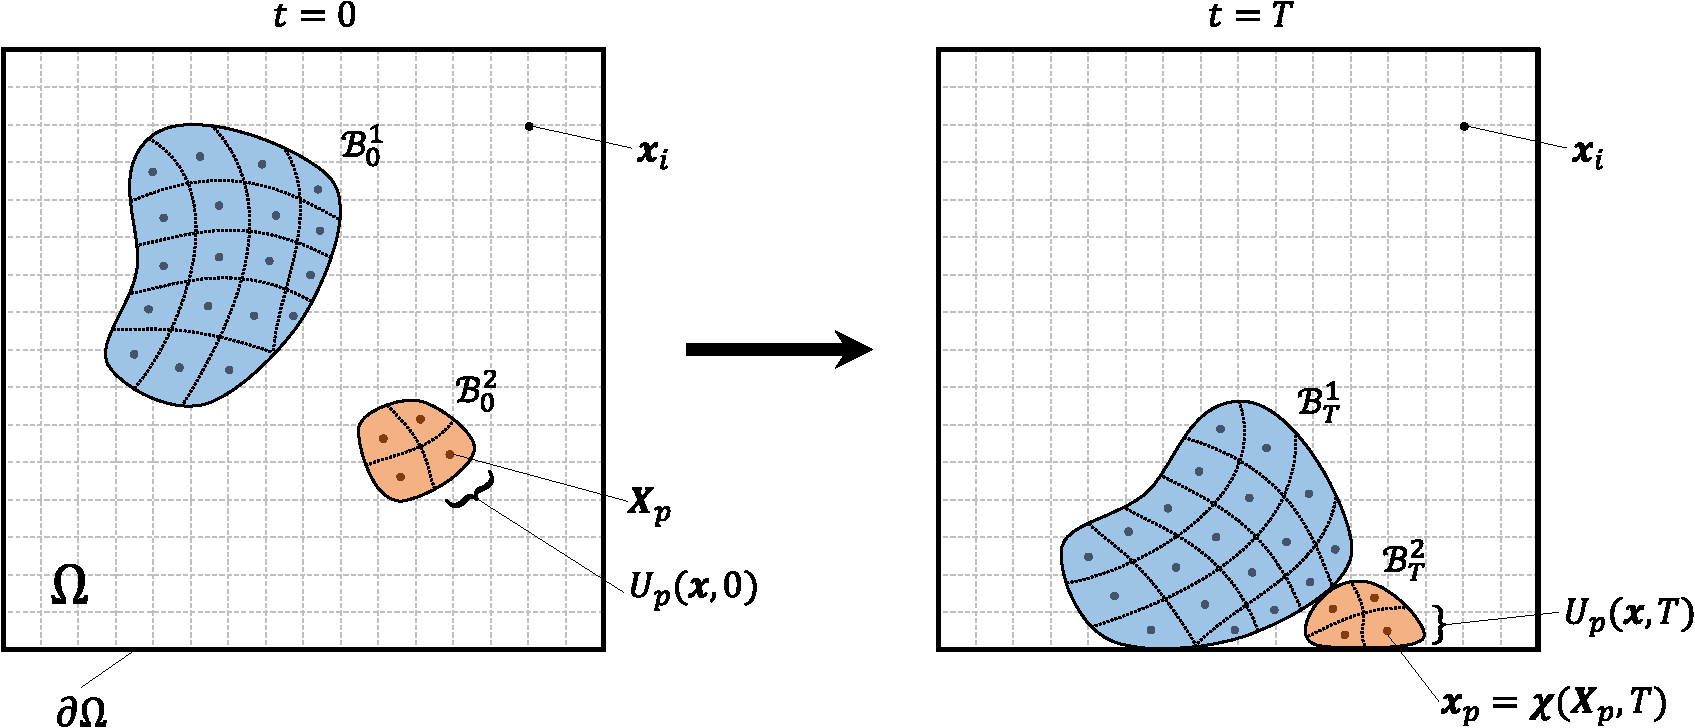
\includegraphics[scale=0.5]{images/SimulationDiagram.pdf}
\caption{Pictorial representation of a material point method simulation for two bodies, $\mathcal{B}^1$ and $\mathcal{B}^2$, in a 2D square domain $\Omega$ from $t=0$ to $t=T$. Each body is simulated by integrating \eqref{eq:pde} through time according to the relevant constitutive laws defined on each body, the initial state of the bodies ($\mathcal{B}_0^1$ and $\mathcal{B}_0^2$), and the boundary conditions defined on $\partial \Omega$, $\partial \mathcal{B}^1$, and $\partial{B}^2$. In this representation, the kinematic fields are discretized on a cartesian grid with functions defined for each node $i$ and the remaining fields are defined on the point function space $U_p(\Vector{x}, t)$ centered on each material point $p$.} \label{fig:simulation}
\end{figure}

\section{Points File}
To integrate the PDEs in \eqref{eq:pde} through time, \texttt{mpm\_3d} needs to define a set of initial conditions. In its default configuration, \texttt{mpm\_3d} will do this by reading a space-delimited points file with the following form,
\lstset{language=C++,
                basicstyle=\ttfamily,
                keywordstyle=\color{blue}\ttfamily,
                stringstyle=\color{red}\ttfamily,
                commentstyle=\color{green}\ttfamily,
                morecomment=[l][\color{magenta}]{\#}
}
\begin{lstlisting}[language={}, escapeinside={(*}{*)}]
    (*$N$*)
    (*$m_1$*) (*$v_1$*) (*$\Vector{X_1}$*) (*$\Vector{v_1}$*) 1
    (*$m_2$*) (*$v_2$*) (*$\Vector{X_2}$*) (*$\Vector{v_2}$*) 1
    ...
    (*$m_N$*) (*$v_N$*) (*$\Vector{X_N}$*) (*$\Vector{v_N}$*) 1
\end{lstlisting}
where the sets of coefficients \(\{m_p\}\), \(\{v_p\}\), \(\{\Vector{X_p}\}\), and \(\{\Vector{v_p}\}\) are defined as follows,
\[
\begin{aligned}
m_p &= \int_{\Omega}{\rho_p U_p(\Vector{x},0) dv}
\\v_p &= \int_{\Omega}{U_p(\Vector{x},0) dv}
\\\Vector{X_p} &= \frac{1}{m_p}\int_{\Omega}{\rho_p \Vector{x} U_p(\Vector{x},0) dv}
\\\Vector{v_p} &= \frac{1}{m_p}\int_{\Omega}{\rho_p \Vector{v}(\Vector{x},0) U_p(\Vector{x},0) dv}
\end{aligned}
\]

\texttt{mpm\_3d} can be run in 1D (uniaxial-strain), 2D (plane-strain or axisymmetric), or 3D. Defining the dimension of a simulation will be covered in more detail in section \ref{scn:config_file}; however, the number of coefficients that define the set of vectors \(\{\Vector{X_p}\}\) or \(\{\Vector{v_p}\}\) in the points file will change according to the choice of simulation dimension.

To generate a points file, there are a number of poorly commented python scripts in the \texttt{mpm\_pygen} folder. In particular, any python script ending in `\texttt{\_v2}' will provide a good starting point for generating your own files.


\section{Output Directory}
While \texttt{mpm\_3d} is running, it will output simulation snapshots. By default, these simulation snapshots are saved as individual `\texttt{.vtk}' files. It is often useful to direct these files to an new output directory.

\texttt{\$ mkdir output}


\section{Configuration File} \label{scn:config_file}
The last step in setting up a simulation for \texttt{mpm\_3d} is the creation of a configuration file. The configuration file contains information about the various objects and parameters that \texttt{mpm\_3d} will need to create to run the simulation. A pictorial representation of the structure of these objects is shown in figure \ref{fig:code}. A comprehensive list of currently implemented objects/classes can be found in section \ref{scn:udc}.

\begin{figure}[!ht]
\centering
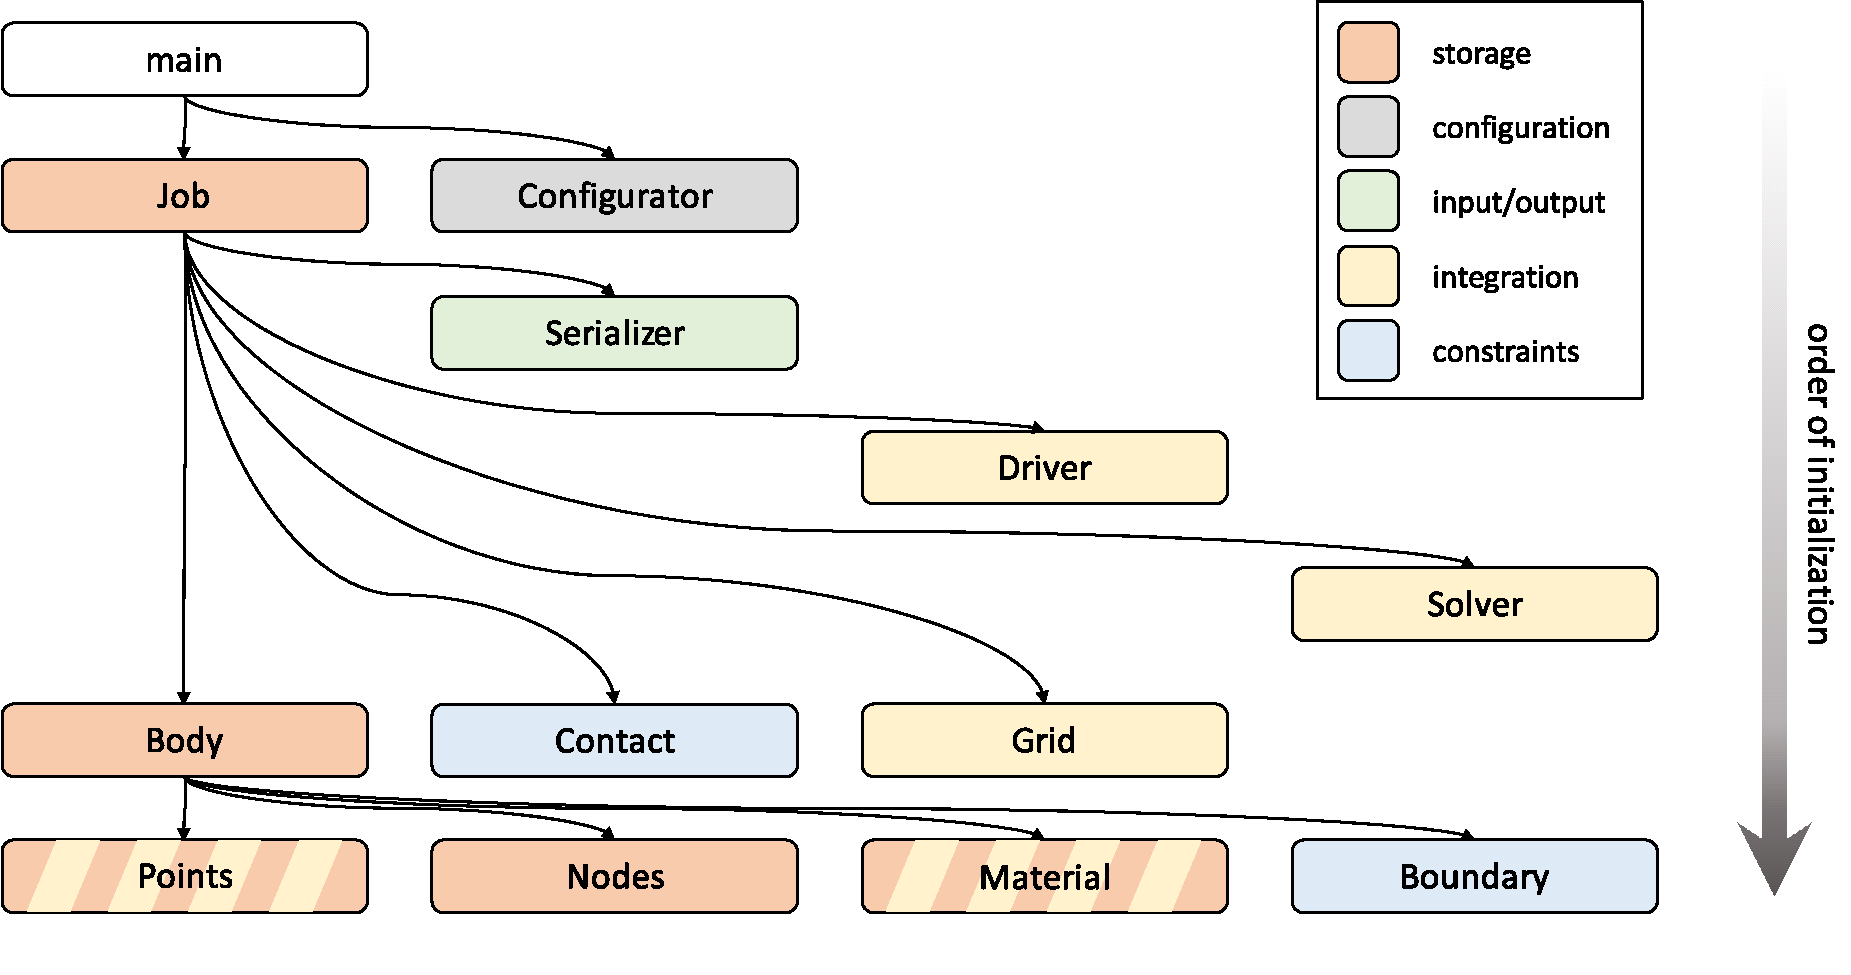
\includegraphics[scale=0.5]{images/CodeDiagram.pdf}
\caption{Pictorial representation of object structure within \texttt{mpm\_3d}. When \texttt{mpm\_3d} is called, the \texttt{main} function creates a \texttt{Job} and \texttt{Configurator} object. The \texttt{Configurator} parses the configuration file described in section \ref{scn:config_file} and initializes the \texttt{Job} object. The \texttt{Job} object stores all of information and objects needed to run a simulation; each \texttt{Job} object has a \texttt{Serializer} for writing outputs, a \texttt{Driver} for integrating time $t$, a \texttt{Solver} for integrating the PDEs in \eqref{eq:pde} through a single time increment, a \texttt{Grid} for integrating nodal basis functions, a set of \texttt{Body} objects, and a set of \texttt{Contact} objects. The \texttt{Body} object stores the information and objects for simulating a single continuum body; each \texttt{Body} object has a \texttt{Points} object for storing point coefficients and integrating point basis functions, a \texttt{Nodes} object for storing node coefficients, a \texttt{Material} for storing material states and integrating stresses through a single time increment, and a \texttt{Boundary} for enforcing constraints on the simulation domain boundary $\partial \Omega$. Each \texttt{Contact} enforces constraints for interactions between \texttt{Body} objects within the simulation domain $\Omega$.} \label{fig:code}
\end{figure}

Every configuration file begins with the definition of the `\texttt{job}' object as follows,
\begin{lstlisting}[language={}, escapeinside={(*}{*)}]
    job
    {
        t = 0
        dt = 1e-3
        TYPE = 2
    }
\end{lstlisting}
The `\texttt{t}' parameter denotes the start time for the simulation and the `\texttt{dt}' parameter denotes the length of the discrete time integration steps. (Note that all parameters are assumed to be defined in terms of kilograms, meters, and seconds.)

The `\texttt{TYPE}' parameter is an integer between 1 and 5 that defines the type of simulation. \texttt{1} is used for 1D (uniaxial-strain) simulations, \texttt{2} is used for 2D (plane-strain) simulations, \texttt{3} is used for 3D simulations, \texttt{4} is used for axisymmetric simulations, and \texttt{5} is used for 2D simulations with out-of-plane motion.

This is followed by the definition of a `\texttt{serializer}' object,
\begin{lstlisting}[language={}, escapeinside={(*}{*)}]
    serializer
    {
        class = "DefaultVTK"
        #frames-per-second
        properties = {60}
        int-properties = {}
        #{output-dir, save-dir, sim-name}
        str-properties = {"output", "save", "example"}
    }	
\end{lstlisting}
The `\texttt{serializer}' is the first object that can be user-defined and governs the input/output behavior of \texttt{mpm\_3d}. Here the `\texttt{DefaultVTK}' serializer class is implemented. A complete list of serializer options and definitions can be found in section \ref{scn:serializers}. The `\texttt{properties}' keyword takes in a comma-separated list of floating-point numbers, which for `\texttt{DefaultVTK}' is a single value for the rate at which simulation snapshots are saved. The `\texttt{int-properties}' keyword takes in a comma-separated list of integers (which is left empty for `\texttt{DefaultVTK}'), and the `\texttt{str-properties}' keyword takes in a comma-separated list of strings, which for `\texttt{DefaultVTK}' is the output directory for the simulation snapshots, a non-implemented save directory, and a simulation name. (Note that comments can be written in the configuration file using `\texttt{\#}' symbol.)

The `\texttt{driver}' object is defined with a similar structure to the `\texttt{serializer}' object as follows,
\begin{lstlisting}[language={}, escapeinside={(*}{*)}]
    driver
    {
        class = "DefaultDriver"
        properties = {1}
        int-properties = {}
        str-properties = {}
    }
\end{lstlisting}
The `\texttt{driver}' object acts like a while-loop for time-integration; it will call the `\texttt{solver}' to integrate the system of equations in \eqref{eq:pde} during each time-step until the simulation has completed. Here the `\texttt{DefaultDriver}' driver class is implemented. A complete list of driver options can be found in section \ref{scn:drivers}. `\texttt{DefaultDriver}' requires only one `\texttt{properties}' item, the stop time for the simulation.

Now the `\texttt{solver}' object is defined,
\begin{lstlisting}[language={}, escapeinside={(*}{*)}]
    solver
    {
        class = "ExplicitUSL"
        properties = {}
        int-properties = {1, 1}
        str-properties = {}
    }
\end{lstlisting}
As stated above, the `\texttt{solver}' object integrates the system of equations in \eqref{eq:pde} through one time-step. The class `\texttt{ExplicitUSL}' implements a forward euler integration scheme. A complete list of solver options can be found in section \ref{scn:solvers}.

The next item in the configuration file is the `\texttt{grid}' object,
\begin{lstlisting}[language={}, escapeinside={(*}{*)}]
    grid
    {
        class = "CartesianLinear"
        #Lx, Ly
        properties = {1.0, 1.0}
        #Nx, Ny
        int-properties = {20, 20}
        str-properties = {}
    }
\end{lstlisting}
The `\texttt{grid}' object defines the simulation domain and nodal function space used to discretize the kinematic fields in the simulation. The `\texttt{CartesianLinear}' grid class defines linear (for \texttt{TYPE = 1}), bi-linear (for \texttt{TYPE = 2}, \texttt{4}, or \texttt{5}), or tri-linear (for \texttt{TYPE = 3}) functions on a cartesian grid. The side lengths of the grid are given by the `\texttt{properties}' keyword and the number of linear elements on each edge are given by the `\texttt{int-properties}' keyword. A complete list of grid options can be found in section \ref{scn:grids}.

The next objects to be defined in the configuration file are the `\texttt{body}' objects,
\begin{lstlisting}[language={}, escapeinside={(*}{*)}]
    body
    {
        class = "DefaultBody"
        name = "block_0"
        properties = {}
        int-properties = {}
        str-properties = {}
        point-file = "block_0.points"

        point-class = "DefaultPoints"
        point-props = {}
        point-int-props = {}
        point-str-props = {}

        node-class = "DefaultNodes"
        node-props = {}
        node-int-props = {}
        node-str-props = {}
        
        material-class = "IsotropicLinearElasticity"
        #{E, (*$\nu$*)}
        material-props = {1e5,0.3}
        material-int-props = {}
        material-str-props = {}
        
        boundary-class = "CartesianBox"
        boundary-props = {}
        boundary-int-props = {}
        boundary-str-props = {}
    }
    
    body
    {
        class = "DefaultBody"
        name = "block_1"
        point-file = "block_1.points"
        
        point-class = "DefaultPoints"
        node-class = "DefaultNodes"    

        material-class = "IsotropicLinearElasticity"
        material-props = {1e8,0.4}
        
        boundary-class = "CartesianBox"
    }
\end{lstlisting}
The `\texttt{body}' objects represent continuum bodies within the simulated domain. (Note that multiple bodies can be simulated at the same time). Here the `\texttt{DefaultBody}' class is implemented. Each body is assigned a \textit{unique} `\texttt{name}' and points file (using the `\texttt{point-file}' keyword). As stated above, the points file contains the initial conditions for the continuum body. In addition, each `\texttt{body}' definition contains a `\texttt{node-class}', `\texttt{point-class}', `\texttt{material-class}', and `\texttt{boundary-class}'. The `\texttt{point-class}' (here set to `\texttt{DefaultPoints}') and `\texttt{node-class}' (here set to `\texttt{DefaultNodes}') are containers for the coefficients defining the point and node fields respectively. The `\texttt{material-class}', here set to `\texttt{IsotropicLinearElasticity}', defines the update rule for the stress in the body as given by the expression,
\begin{equation} \label{eq:stress_pde}
\dot{\Tensor{\sigma}} = \hat{\dot{\Tensor{\sigma}}}(\Tensor{\varepsilon},\dot{\Tensor{\varepsilon}},\Tensor{w},\Tensor{\sigma},\xi)
\end{equation}
The `\texttt{boundary-class}', here set to `\texttt{CartesianBox}', defines the boundary conditions for the body. A full list of body, points, nodes, material, and boundary options can be found in section \ref{scn:udc}.

The final objects defined in the configuration file are the `\texttt{contact}' objects,
\begin{lstlisting}[language={}, escapeinside={(*}{*)}]
    contact
    {
        name = "collision"
        class = "ContactHuang"
        properties = {0.4}
        int-properties = {}
        str-properties = {"block_0","block_1"}
    }
\end{lstlisting}
The `\texttt{contact}' object, here set to `\texttt{ContactHuang}', defines the kinematic constraints on bodies due to their interactions with other bodies in the simulation. The `\texttt{ContactHuang}' contact class implements the constraints given in \cite{huang2011} and takes in a single floating point property and two string properties (the coefficient of friction between the two bodies and the `\texttt{name}' of the bodies). If more than one contact rule is given (required if there are more than two bodies in a simulation), then the constraints will be applied in the order they appear in the configuration file. A full list of contact options can be found in section \ref{scn:contacts}.

If everything has been written correctly (including the points files), then the simulation should be ready to run!

\section{Calling Program}
To run the simulation, simply call \texttt{mpm\_v3} from the command line as follows,

\texttt{\$ ./mpm\_v3 -c CONFIGURATION-FILE}

The `\texttt{-c}' flag calls \texttt{mpm\_3d} to read the configuration file as input for the simulation. Other options may be implemented in the future.


\section{Visualizing Results}
The default output from \texttt{mpm\_3d} is a series of simulation snapshots in the form of `\texttt{.vtk}' files. There are several open-source software packages which can be used to view and interact with the data in these files including ParaView by Kitware and VisIt by Lawrence Livermore National Labs.